\chapter{Teorie modelů}\label{chapter:model-theory}

V této kapitole se trochu vzdálíme typickým aplikacím logiky v informatice\footnote{Například použití rezoluce k řešení otázky, zda v dané konečné teorii $T$ platí daná sentence $\varphi$.} a nahlédneme o úroveň abstrakce výše, do oblasti \emph{matematické} logiky. \emph{Teorie modelů} se snaží popsat vztah mezi obecnými vlastnostmi teorií (predikátové logiky) a tříd jejich modelů. Nevyhneme se práci s nekonečnými teoriemi a s nekonečnými strukturami. Jde jen o ukázku několika vybraných výsledků, které jsou pro nás dostupné. Ani se nepokusíme obsáhnout všechny hlavní oblasti teorie modelů, která je velmi bohatá a hluboká. Do této kapitoly jsme také přidali materiál týkající se vlastností modelů, který se nehodil jinam.


\section{Elementární ekvivalence}

Nejprve se podíváme na několik vlastností souvisejících s pojmem \emph{elementární ekvivalence}. Připomeňme, že $L$-struktury $\A$ a $\B$ jsou \emph{elementárně ekvivalentní} ($\A\equiv \B$), pokud v nich platí tytéž $L$-sentence.

V teorii modelů nás často zajímá, jaké vlastnosti (sentence) platí v dané, konkrétní struktuře:

\begin{definition}[Teorie struktury]
Mějme $L$-strukturu $\A$. \emph{Teorie struktury} $\A$, značíme $\Th(\A)$ je množina všech $L$-sentencí platných v $\A$:
$$
\Th(\A)=\{\varphi\mid\varphi\text{ je $L$-sentence a }\A\models\varphi\}
$$
\end{definition}

\begin{example}
Jako důležitý příklad vezměme \emph{standardní model aritmetiky}, strukturu $\underline{\mathbb{N}}=\langle\mathbb{N},S,+,\cdot,0,\le\rangle$. Teorii $\Th(\underline{\mathbb{N}})$ říkáme \emph{aritmetika přirozených čísel}. V následující kapitole si ukážeme, že je \emph{(algoritmicky) nerozhodnutelná}.\footnote{Teorie $T$ je \emph{(algoritmicky) rozhodnutelná}, pokud existuje algoritmus, který pro každou vstupní sentenci $\varphi$ doběhne a odpoví, zda $T\models\varphi$.}
\end{example}

Několik jednoduchých vlastností teorie struktury shrneme v následujícím pozorování:

\begin{observation}
    Nechť $\A$ je $L$-struktura a $T$ je $L$-teorie.
    \begin{enumerate}[(i)]
        \item Teorie $\Th(\A)$ je kompletní.
        \item Je-li $\A\in\M_L(T)$, potom $\Th(\A)$ je (kompletní) jednoduchá extenze teorie $T$.
        \item Pokud $\A\in\M_L(T)$ a $T$ je kompletní, potom je $\Th(\A)$ ekvivalentní s $T$, v tom případě $\Th(\A)=\Conseq_L(T)$.
        
    \end{enumerate}    
\end{observation}

Pomocí pojmu \emph{teorie struktury} můžeme také vyjádřit elementární ekvivalenci, pro $L$-struktury $\A,\B$ platí:
$$
\A\equiv\B \text{ právě když }\Th(\A)=\Th(\B).
$$

\begin{example}
   Podívejme se standardní uspořádání reálných, racionálních, a celých čísel, tj. na struktury $\langle\mathbb R,\leq\rangle$, $\langle\mathbb Q,\leq\rangle$, $\langle\mathbb Z,\leq\rangle$. Jak jsme již zmínili v Příkladu \ref{example:elementary-equivalence-of-orders-R-Q}, není těžké ukázat, že $\langle\mathbb R,\leq\rangle\equiv\langle\mathbb Q,\leq\rangle$ (pomocí \emph{hustoty} těchto uspořádání). Struktury $\langle\mathbb Q,\leq\rangle$ a $\langle\mathbb Z,\leq\rangle$ ale elementárně ekvivalentní nejsou: V $\langle\mathbb Z,\leq\rangle$ má každý prvek bezprostředního následníka, což v $\langle\mathbb Q,\leq\rangle$ neplatí. Pro následující sentenci $\varphi$ tedy máme $\varphi\in\Th(\langle\mathbb Z,\leq\rangle)$ ale $\varphi\not\in\Th(\langle\mathbb Q,\leq\rangle)$:
   $$
   \varphi=(\forall x)(\exists y)(x\leq y\land \neg x=y\land(\forall z)(x\leq z\limplies z=x\lor y\leq z)
   $$
\end{example}


\subsection{Kompletní jednoduché extenze}

Máme-li teorii $T$, zajímá nás, jak vypadají její modely. Připomeňme, že:
\begin{itemize}
    \item Teorie je \emph{kompletní}, právě když má jediný model až na elementární ekvivalenci.\footnote{Tedy všechny její modely jsou elementárně ekvivalentní.}
    \item Modely teorie $T$ až na elementární ekvivalenci jednoznačně odpovídají kompletním jednoduchým extenzím $T$.
\end{itemize}
Kompletní jednoduché extenze $L$-teorie $T$ jsou tedy tvaru $\Th(\A)$ pro $\A\in\M_L(T)$, a (jak jsme už zmínili výše) $\A\equiv\B$ právě když $\Th(\A)=\Th(\B)$. Místo hledání všech modelů tedy stačí najít všechny kompletní jednoduché extenze.

\begin{proposition}\label{propositon:efficient-complete-simple}    
    Pokud lze \emph{efektivně (algoritmicky) popsat} všechny kompletní jednoduché extenze\footnote{Představte si algoritmus, který pro daná vstupní $i,j$ odpoví $j$-tý axiom $i$-té kompletní jednoduché extenze (v nějakém pevném očíslování); takový algoritmus ne vždy existuje!} \emph{efektivně dané} teorie $T$,\footnote{$T$ může být nekonečná, ale musí existovat algoritmus, který generuje všechny axiomy $T$.} potom je $T$ \emph{(algoritmicky) rozhodnutelná}.
\end{proposition}
\begin{proof}
Pro danou sentenci $\varphi$ buď $T\proves\varphi$, nebo existuje protipříklad $\A\not\models\varphi$, tedy kompletní jednoduchá extenze $T_i$ teorie $T$ taková, že $T_i\not\proves\varphi$. Z kompletnosti ale plyne, že $T_i\proves\neg\varphi$. Náš algoritmus bude paralelně konstruovat tablo důkaz $\varphi$ z $T$ a tablo důkaz $\neg\varphi$ ze všech kompletních jednoduchých extenzí $T_1,T_2,\dots$ teorie $T$.\footnote{Nevadí, že je jich nekonečně mnoho, můžeme využít tzv. \emph{dovetailing}: Provedeme 1. krok konstrukce 1. tabla, potom 2. krok 1. tabla a 1. krok 2. tabla, 3. krok 1. tabla, 2. krok 2. tabla, 1. krok 3. tabla, atd.} Víme, že alespoň jedno z paralelně konstruovaných tabel je sporné, a můžeme předpokládat, že konečné (neprodlužujeme-li sporné větve tabla), tedy algoritmus ho po konečně mnoha krocích zkonstruuje.
\end{proof}

Schopnost efektivně popsat všechny kompletní jednoduché extenze je poměrně vzácná, a vyžaduje silné předpoklady. Přesto to lze provést u mnoha důležitých teorií. Uveďme jeden příklad: \emph{teorii hustého lineárního uspořádání (dense linear order)}.

\subsubsection{Příklad: DeLO*}

Teorie \emph{hustého lineárního uspořádání (DeLO*)}  je extenze teorie uspořádání o následující axiomy: 
\begin{itemize}
    \item axiom \emph{linearity} (někdy se mu říká také \emph{dichotomie}):
    $$
    x\leq y\lor y\leq x
    $$
    \item axiom \emph{hustoty}
    $$
    {x\leq y}\land{\neg\,x=y}\limplies(\exists z)(x\leq z\land z\leq y\land\neg\,z=x\land\neg\,z=y)
    $$
\end{itemize}
Někdy se přidává i axiom \emph{netriviality} $(\exists x)(\exists y)(\neg\,x=y)$ zakazující jednoprvkový model. Tato teorie není kompletní, umíme ale popsat všechny její kompletní jednoduché extenze:

\begin{proposition}
Mějme sentence $\varphi=(\exists x)(\forall y)(x\leq y)$ a $\psi=(\exists x)(\forall y)(y\leq x)$ vyjadřující existenci minimálního resp. maximálního prvku. Následující čtyři teorie jsou právě všechny kompletní jednoduché extenze teorie DeLO*:
\begin{itemize}
    \item $\DeLO = \DeLO^*\ \cup \ \{\neg\varphi
    ,\neg\psi\}$
    \item $\DeLO^+ = \DeLO^*\ \cup \ \{\neg\varphi
    ,\psi\}$
    \item $\DeLO^- = \DeLO^*\ \cup \ \{\varphi
    ,\neg\psi\}$
    \item $\DeLO^\pm = \DeLO^*\ \cup \ \{\varphi
    ,\psi\}$        
\end{itemize}
\end{proposition}

Stačí ukázat, že tyto čtyři teorie jsou kompletní. Potom už je zřejmé, že žádná další kompletní jednoduchá extenze DeLO* nemůže existovat. Jak vysvětlíme v Sekci \ref{section:categoricity}, jejich kompletnost plyne z faktu, že jsou \emph{$\omega$-kategorické}, tj. mají jediný spočetný model až na elementární ekvivalenci. 

Z Tvrzení \ref{propositon:efficient-complete-simple} potom plyne rozhodnutelnost:

\begin{corollary}
    Teorie DeLO* je (algoritmicky) rozhodnutelná.
\end{corollary}


\subsection{Důsledky Löwenheim-Skolemovy věty}

V Sekci \ref{subsection:loewenheim-skolem-theorem} jsme dokázali tzv. Löwenheim-Skolemovu větu, konkrétně její variantu pro jazyky bez rovnosti:

\begin{theorem-unnumbered}[Löwenheim-Skolemova]
    Je-li $L$ spočetný jazyk bez rovnosti, potom každá bezesporná $L$-teorie má spočetně nekonečný model.
\end{theorem-unnumbered}

Tato věta má následující jednoduchý důsledek:

\begin{corollary}\label{corollary:loewenheim-skolem-without-equality}
    Je-li $L$ spočetný jazyk bez rovnosti, potom ke každé $L$-struktuře existuje elementárně ekvivalentní spočetně nekonečná struktura.
\end{corollary}
\begin{proof}
    Mějme $L$-strukturu $\A$. Teorie $\Th(\A)$ je bezesporná (má model $\A$), tedy dle Löwenheim-Skolemovy má spočetně nekonečný model $\B\models\Th(\A)$. To ale znamená, že $\B\equiv\A$.
\end{proof}
V jazyce bez rovnosti tedy nemůžeme vyjádřit například `model má právě 42 prvků'.

V důkazu Löwenheim-Skolemovy věty jsme sestrojený model získali jako kanonický model pro bezespornou větev tabla z $T$ pro položku $\F\bot$. Stejným způsobem se dokáže následující verze pro jazyky s rovností, stačí faktorizovat dle relace $=^A$:

\begin{theorem-unnumbered}[Löwenheim-Skolemova s rovností]
    Je-li $L$ spočetný jazyk s rovností, potom každá bezesporná $L$-teorie má spočetný model (tj. konečný, nebo spočetně nekonečný).
\end{theorem-unnumbered}

I tato verze má snadný důsledek pro konkrétní struktury:

\begin{corollary}\label{corollary:loewenheim-skolem-with-equality}
    Je-li $L$ spočetný jazyk s rovností, potom ke každé \emph{nekonečné} $L$-struktuře existuje elementárně ekvivalentní spočetně nekonečná struktura.
\end{corollary}
\begin{proof}
    Mějme nekonečnou $L$-strukturu $\A$. Stejně jako v důkazu Důsledku \ref{corollary:loewenheim-skolem-without-equality} najdeme spočetně nekonečnou strukturu $\B\equiv\A$. Protože v $\A$ neplatí pro žádné $n\in\mathbb N$ sentence vyjadřující `existuje nejvýše $n$ prvků' (což lze pomocí rovnosti snadno zapsat), neplatí tato sentence ani v $\B$, $\B$ tedy nemůže být konečná struktura.
\end{proof}

Tento důsledek použijeme, abychom ukázali, že existuje spočetné těleso, které je algebraicky uzavřené:  

\subsubsection*{Spočetné algebraicky uzavřené těleso}

Těleso $\A$ je \emph{algebraicky uzavřené}, pokud každý polynom nenulového stupně v něm má kořen. Těleso reálných čísel $\mathbb R$ není algebraicky uzavřené, neboť $x^2+1$ nemá v $\mathbb R$ kořen, stejně tak těleso $\mathbb Q$ (v něm nemá kořen ani $x^2-2$). Těleso komplexních čísel $\mathbb C$ algebraicky uzavřené je, je ale nespočetné.

Algebraickou uzavřenost lze vyjádřit pomocí následujících sentencí $\psi_n$, pro každé $n>0$:
$$
(\forall x_{n-1})\dots(\forall x_0)(\exists y)(y^n+x_{n-1}\cdot y^{n-1}+\dots+x_1\cdot y + x_0 = 0
$$
kde $y^k$ je zkratka za term $y\cdot y \cdot\ \cdots\ \cdot y$ (kde  $\cdot$ je aplikováno ($k-1$)-krát).

\begin{corollary}
    Existuje spočetné algebraicky uzavřené těleso.
\end{corollary}
\begin{proof}
    Dle Důsledku \ref{corollary:loewenheim-skolem-with-equality} existuje spočetně nekonečná struktura $\A$ elementárně ekvivalentní tělesu $\mathbb C$. Protože $\mathbb C$ je těleso a splňuje sentence $\psi_n$ pro všechna $n>0$, je i $\A$ algebraicky uzavřené těleso.
\end{proof}


\section{Izomorfismus struktur}\label{section:isomorphism-of-structures}\todo

% from slides:
\subsubsection*{Izomorfismus struktur}
    %{\it Následující pojem vyjadřuje ``stejnost'' až na přejmenování prvků.}
    %\medskip
    
    Nechť $\mathcal{A}$, $\mathcal{B}$ jsou struktury jazyka $L=\langle\mathcal{F},\mathcal{R}\rangle$.
    \smallskip
    
    \begin{itemize}
    \item \myblue{Bijekce} $h\colon A\to B$ je \mdef{izomorfismus} struktur $\mathcal{A}$ a $\mathcal{B}$, pokud platí zároveň
    \vspace{-2mm}
    \begin{align*}\myblue{(i)}\quad&\mygreen{h(f^A(a_1,\dots,a_n))=f^B(h(a_1),\dots,h(a_n))}\\
    &\text{pro každý $n$-ární funkční symbol $f\in \mathcal{F}$ a každé $a_1,\dots,a_n\in A$,\qquad}\\
    \myblue{(ii)}\quad&\mygreen{R^A(a_1,\dots,a_n)\ \ \Leftrightarrow\ \ R^B(h(a_1),\dots,h(a_n))}\\
    &\text{pro každý $n$-ární relační symbol $R\in \mathcal{R}$ a každé $a_1,\dots,a_n\in A$.}
    \end{align*}
    
    \vspace{-1mm}
    \item $\mathcal{A}$ a $\mathcal{B}$ jsou \mdef{izomorfní} (via $h$), psáno \mdef{$\mathcal{A}\simeq\mathcal{B}$} ($\mathcal{A}\simeq_h\mathcal{B}$), pokud existuje
        \smallskip
    
        izomorfismus $h$ struktur $\mathcal{A}$ a $\mathcal{B}$. Říkáme rovněž, že $\mathcal{A}$ je \mdef{izomorfní s} $\mathcal{B}$.
    \smallskip
    
    \item \mdef{Automorfismus} struktury $\mathcal{A}$ je izomorfismus $\mathcal{A}$ s $\mathcal{A}$.
    \end{itemize}
    \medskip
    
    \mygreen{\it Např. potenční algebra $\underline{\mathcal{P}(X)}=\langle \mathcal{P}(X),-,\cap,\cup,\emptyset,X\rangle$ s $X=n$ je izomorfní}
    \smallskip
    
    \mygreen{\it s Booleovou algebrou $\underline{^{n}2}=\langle ^{n}2,-_n,\mand_n,\mor_n,0_n,1_n \rangle$ via $h: A \mapsto \chi_A$, kde $\chi_A$}
    \smallskip
    
    \mygreen{\it je charakteristická funkce množiny $A\subseteq X$.} % NeplatíDále $g: A \mapsto \overline{A}$ je automorfismus $\underline{\mathcal{P}(X)}$.}
    
    
    %%%%%%%%%%%%%%%%%%%%%%%%%%%%%%%%%%%%%%%%%%%%%%%%%%%%%%5
    
    \subsubsection*{Izomorfismus a sémantika}
    {\it Uvidíme, že izomorfismus zachovává sémantiku.}
    \medskip
    
    {\bf \myblue{Tvrzení}}\ \ {\it Nechť $\mathcal{A}$, $\mathcal{B}$ jsou struktury jazyka $L=\langle\mathcal{F},\mathcal{R}\rangle$.
    \smallskip
    Bijekce $h\colon A\to B$ je \myblue{izomorfismus} $\mathcal{A}$ a $\mathcal{B}$, právě když platí zároveň
    \vspace{-1mm}
    \begin{align*}\myblue{(i)}\quad&\mygreen{h(t^A[e])=t^B[e\circ h]}& &\text{pro každý term $t$ a $e\colon \mathrm{Var} \to A$, }\\
    %&\text{pro každý $n$-ární funkční symbol $f\in \mathcal{F}$ a každé $a_1,\dots,a_n\in A$,\qquad}\\
    \myblue{(ii)}\quad&\mygreen{\mathcal{A}\models \varphi[e]\ \ \Leftrightarrow\ \ \mathcal{B}\models \varphi[e\circ h]}&\quad &\text{pro každou formuli $\varphi$ a $e\colon \mathrm{Var} \to A$.}\qquad
    \end{align*}}
    
    {\it \myblue{Důkaz}}\ \ ($\Rightarrow$)\ \ Indukcí dle struktury termu $t$, respektive formule $\varphi$.
    \smallskip
    
    ($\Leftarrow$)\ \ Dosazením termu $f(x_1,\dots,x_n)$ do $(i)$ či atomické formule $R(x_1,\dots,x_n)$
    \smallskip
    
    do $(ii)$ pro ohodnocení $e(x_i)=a_i$ máme, že $h$ vyhovuje def. izomorfismu.$\qed$
    \bigskip
    
    {\bf \myblue{Důsledek}}\ \ {\it Pro každé struktury $\mathcal{A}$, $\mathcal{B}$ stejného jazyka,}
    \vspace{-2mm}
    \mygreen{$$\mathcal{A}\simeq\mathcal{B}\ \ \Rightarrow\ \ \mathcal{A}\equiv\mathcal{B}.$$}
    
    \vspace{-6mm}
    {\it \myblue{Poznámka}}\ \ {\it Obrácená implikace \myblue{obecně} neplatí, např. \mygreen{$\langle \mathbb{Q},\le \rangle\equiv \langle \mathbb{R},\le\rangle$}, ale
    \smallskip
    
    \mygreen{$\langle \mathbb{Q},\le \rangle\not\simeq \langle \mathbb{R},\le\rangle$}, neboť $|\mathbb{Q}|=\omega$ a $|\mathbb{R}|=2^\omega$.}
    
    
    %%%%%%%%%%%%%%%%%%%%%%%%%%%%%%%%%%%%%%%%%%%%%%%%%%%%%%5
    
    \subsubsection*{Konečné modely s rovností}
    
    {\bf \myblue{Tvrzení}}\ \ {\it Pro každé \myblue{konečné} struktury $\mathcal{A}$, $\mathcal{B}$ stejného jazyka s \myblue{rovností},}
    \vspace{-2mm}
    \mygreen{$$\mathcal{A}\equiv\mathcal{B}\ \ \Rightarrow\ \ \mathcal{A}\simeq\mathcal{B}.$$}
    
    \vspace{-6mm}
    {\it \myblue{Důkaz}}\ \ Je $|A|=|B|$, neboť lze vyjádřit \emph{``existuje právě $n$ prvků''}.
    \begin{itemize}
    \item Nechť $\mathcal{A}'$ je expanze $\mathcal{A}$ do jazyka $L'=L\cup\{c_a\}_{a\in A}$ o \myblue{jména prvků} z $A$.
    \item Ukážeme, že $\mathcal{B}$ lze expandovat na $\mathcal{B}'$ do jazyka $L'$ tak, že $\mathcal{A}'\equiv \mathcal{B}'$. Pak
    \vspace{0.5mm}
    
    zřejmě $h\colon a \mapsto c_a^{B'}$ je izomorfismus $\mathcal{A}'$ s $\mathcal{B}'$ a tedy i izomorfismus $\mathcal{A}$ s $\mathcal{B}$.
    \item Stačí ukázat, že pro každé $c^{A'}_a=a\in A$ existuje $b\in B$\ \ t.ž. \myblue{$\langle  \mathcal{A},a\rangle\equiv\langle\mathcal{B},b\rangle$}.
    \item Označme $\Omega$ množinu formulí $\varphi(x)$ t.ž. $\langle \mathcal{A},a\rangle \models \varphi(x/c_a)$, tj. $\mathcal{A}\models \varphi[e(x/a)]$.
    \item Jelikož je $A$ konečné, existuje konečně formulí $\varphi_0(x),\dots,\varphi_m(x)$ tak, že
    \vspace{0.5mm}
    
    pro každé $\varphi \in \Omega$ je $\mathcal{A}\models \varphi \leftrightarrow \varphi_i$ pro nějaké $i$.
    \item Jelikož $\mathcal{B}\equiv\mathcal{A}\models (\exists x)\bigwedge_{i\le m}\varphi_i$, existuje $b\in B$ t.ž. $\mathcal{B}\models \bigwedge_{i\le m}\varphi_i[e(x/b)]$.
    \item Tedy pro každou $\varphi\in \Omega$ je $\mathcal{B}\models \varphi[e(x/b)]$, tj. $\langle\mathcal{B},b\rangle\models \varphi(x/c_a)$. $\qed$
    \end{itemize}
    \smallskip
    
    {\bf \myblue{Důsledek}}\ \ {\it Má-li \myblue{kompletní} teorie jazyka s rovností konečný model, jsou
    \vspace{0.5mm}
    
    všechny její modely \myblue{izomorfní}.}
    
% :from slides

\subsection{Definovatelnost a automorfismy}\todo

Připomeňme si pojem definovatelné množiny, viz Sekce \ref{section:definability}.

% from slides:

\subsubsection*{Definovatelnost a automorfismy}
    
    {\it Ukážeme, že definovatelné množiny jsou invariantní na automorfismy.}
    \medskip
    
    {\bf \myblue{Tvrzení}}\ \ {\it Nechť $D\subseteq A^n$ je množina definovatelná ve struktuře $\mathcal{A}$ z parametrů
    \smallskip
    
    $\overline{b}$ a $h$ je \myblue{automorfismus} $\mathcal{A}$, který je \myblue{identický} na $\overline{b}$. Pak $h[D]=D$.}
    \medskip
    
    {\it \myblue{Důkaz}}\ \ Nechť $D=\varphi^{\mathcal{A},\overline{b}}(\overline{x},\overline{y})$. Pak pro každé $\overline{a}\in A^{|\overline{x}|}$
    \vspace{-1mm}
    \begin{align*}\overline{a}\in D\ &\Leftrightarrow\ \mathcal{A}\models \varphi[e(\overline{x}/\overline{a},\overline{y}/\overline{b})]\ \Leftrightarrow\  \mathcal{A}\models \varphi[(e\circ h)(\overline{x}/\overline{a},\overline{y}/\overline{b})]\\
    &\Leftrightarrow\ \mathcal{A}\models \varphi[e(\overline{x}/h(\overline{a}),\overline{y}/h(\overline{b}))]\ \Leftrightarrow\ \mathcal{A}\models \varphi[e(\overline{x}/h(\overline{a}),\overline{y}/\overline{b})]\ \Leftrightarrow\ h(\overline{a})\in D. \qed
    \end{align*}
    \vspace{-4mm}
    
    \mygreen{\it Např. graf $\mathcal{G}$ má právě jeden netriv. automorfismus $h$ zachovávající vrchol $0$.}
    \medskip
    
    \centerline{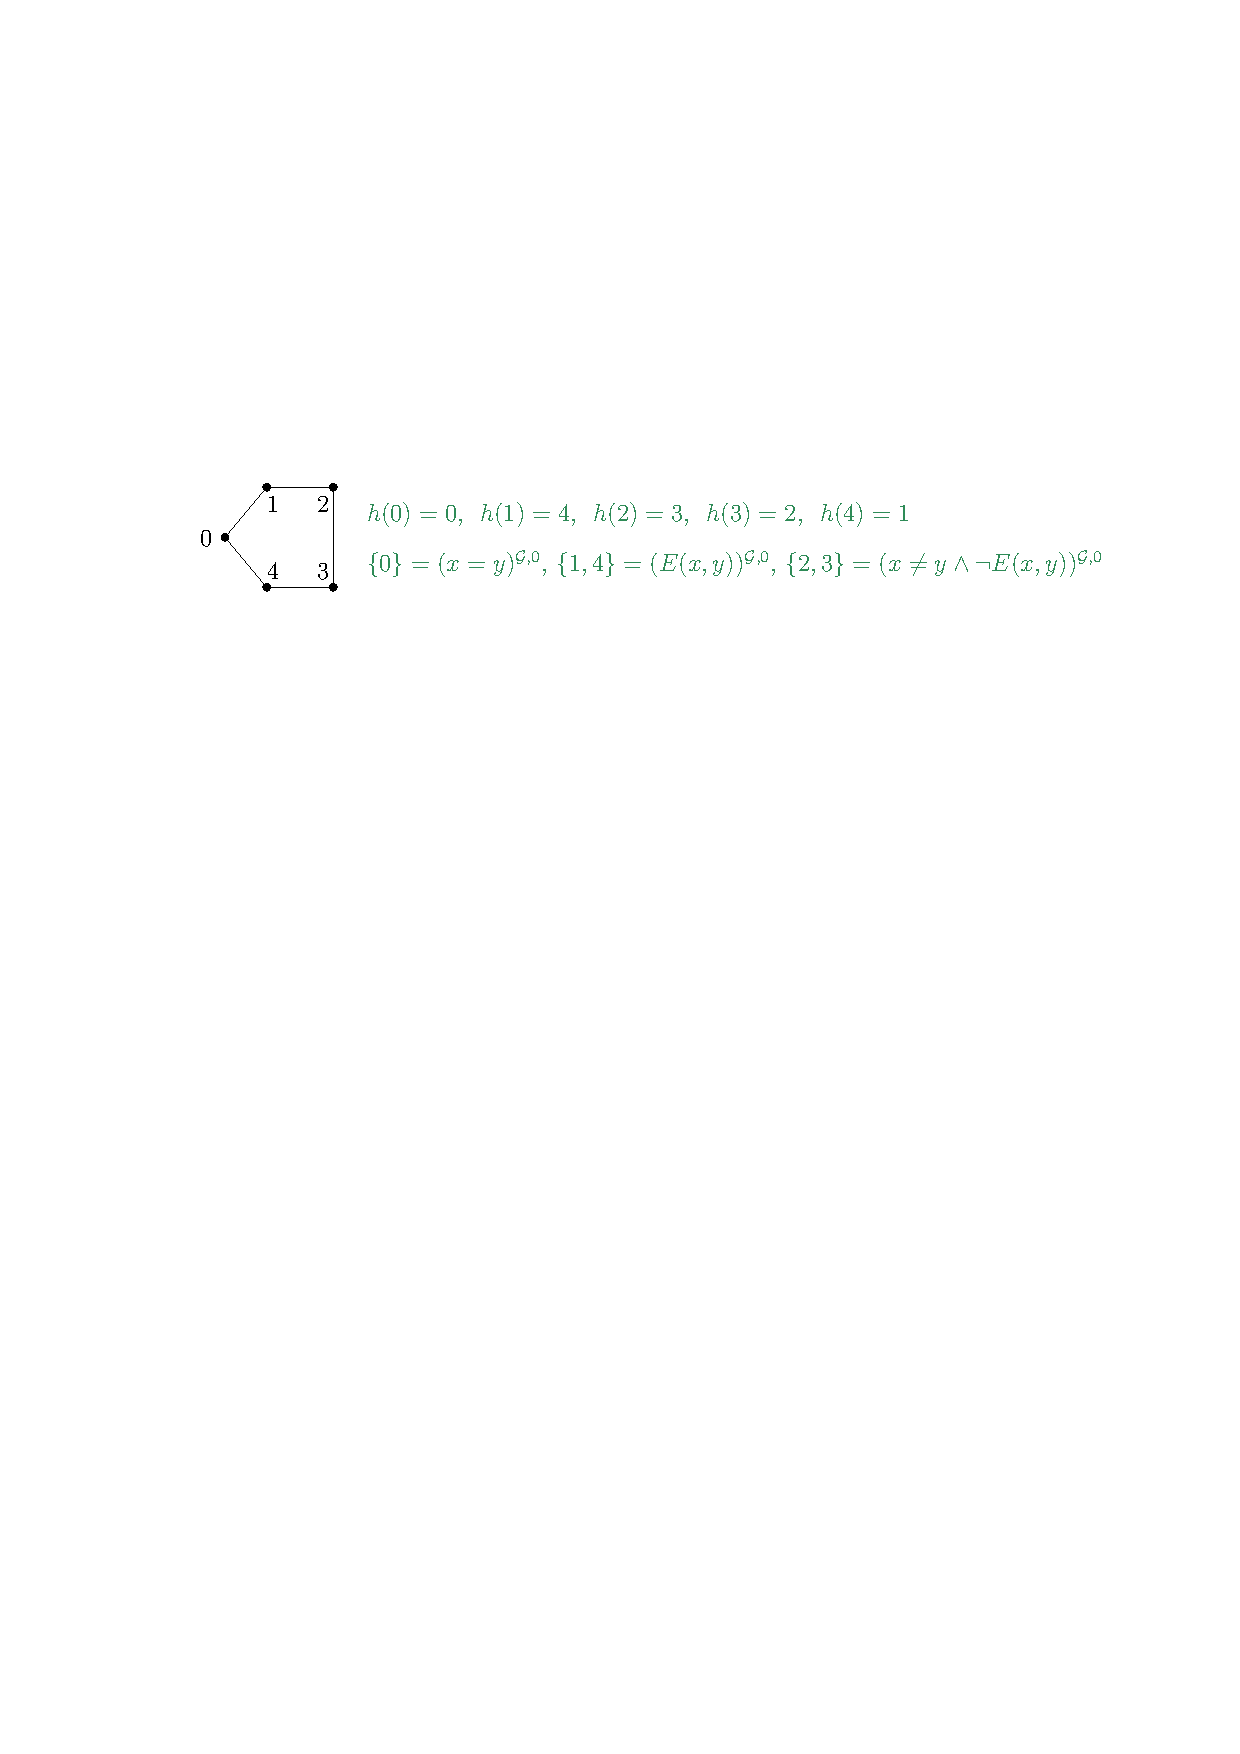
\includegraphics[scale=0.75]{files/5cyklus}}
    \smallskip
    
    \mygreen{\it Navíc množiny $\{0\}$, $\{1,4\}$, $\{2,3\}$ jsou definovatelné z parametru $0$. Tedy
    \vspace{-2mm}
    $$\mathrm{Df}^1(\mathcal{G},\{0\})=\{\emptyset, \{0\}, \{1,4\}, \{2,3\}, \{0,1,4\}, \{0,2,3\}, \{1,4,2,3\}, \{0,1,2,3,4\}\}.$$}
    
    \vspace{-6mm}
    
    
% :from slides

\section{Kategorické teorie}\label{section:categoricity}
\todo

% from slides:
\begin{itemize}
    \item \mdef{Izomorfní spektrum} teorie $T$ je počet \mdef{$I(\kappa,T)$} navzájem neizomorfních
    \smallskip
    
    modelů teorie $T$ pro každou \myblue{kardinalitu} $\kappa$.
        \smallskip
    
    \item Teorie $T$ je \mdef{$\kappa$-kategorická}, pokud má až na izomorfismus právě jeden
    \smallskip
    
    model kardinality $\kappa$, tj. $I(\kappa,T)=1$.
    \end{itemize}
    \medskip
    
    {\bf \myblue{Tvrzení}}\ \ {\it Teorie $DeLO$ \emph{(tj. ``bez konců'')} je $\omega$-kategorická.}
    \medskip
    
    {\it \myblue{Důkaz}}\ \ Nechť $\mathcal{A}$, $\mathcal{B} \models DeLO$ s $A=\{a_i\}_{i\in \mathbb{N}}$, $B=\{b_i\}_{i\in \mathbb{N}}$. Indukcí dle $n$ lze
    \smallskip
    
    nalézt prosté \myblue{parciální} funkce $h_n\subseteq h_{n+1}\subset A\times B$ \myblue{zachovávající uspořádání}
    \smallskip
    
    tak, že $\{a_i\}_{i< n}\subseteq \mathrm{dom}(h_n)$ a $\{b_i\}_{i< n}\subseteq \mathrm{rng}(h_n)$. Pak $\mathcal{A}\simeq \mathcal{B}$ via $h=\cup h_n$. $\qed$
    \bigskip
    
    \mygreen{\it Obdobně dostaneme, že např. $\mathcal{A}=\langle \mathbb{Q},\le\rangle$, $\mathcal{A} \upharpoonright (0,1]$, $\mathcal{A} \upharpoonright [0,1)$, $\mathcal{A} \upharpoonright [0,1]$}
    \smallskip
    
    \mygreen{\it jsou až na izomorfismus všechny spočetné modely teorie $DeLO^*$. Pak}
    \vspace{-2mm}
    \mygreen{$$I(\kappa,DeLO^*)=\begin{cases}0 &\text{pro }\kappa\in\mathbb{N},\\
    4 &\text{pro }\kappa=\omega.\end{cases}$$}
    
    \vspace{-6mm}
% :from slides

\subsection{$\omega$-kategoricita a úplnost}\todo

% from slides:

{\bf \myblue{Věta}}\ \ {\it Nechť jazyk $L$ je spočetný.
\vspace{0.5mm}

\begin{enumerate}
\item[$(i)$] Je-li teorie $T$ jazyka $L$ bez rovnosti $\omega$-kategorická, je kompletní.
\smallskip

\item[$(ii)$] Je-li teorie $T$ jazyka $L$ s rovností $\omega$-kategorická a bez konečného
\smallskip

 modelu, je kompletní.
\end{enumerate}}
\medskip

{\it \myblue{Důkaz}}\ \ Každý model teorie $T$ je elementárně ekvivalentní s nějakým
\smallskip

spočetně nekonečným modelem $T$, ale ten je až na izomorfismus jediný.
\smallskip

Tedy všechny modely $T$ jsou elementárně ekvivalentní, tj. $T$ je kompletní. $\qed$
\bigskip

\mygreen{\it Např. teorie $DeLO$, $DeLO^+$, $DeLO^-$, $DeLO^\pm$ jsou kompletní a jsou to všechny}
\smallskip

\mygreen{\it (navzájem neekvivalentní) jednoduché kompletní extenze teorie $DeLO^*$.}
\bigskip

{\it \myblue{Poznámka}\ \ Obdobné kritérium platí i pro vyšší kardinality než $\omega$.}

% :from slides

\section{Axiomatizovatelnost}\todo

% from slides:

\subsection{Axiomatizovatelnost}
\subsubsection*{Axiomatizovatelnost}

{\it Zajímá nás, zda se daná část světa dá ``dobře'' popsat.}
\medskip

Nechť $K\subseteq M(L)$ je třída struktur jazyka $L$. Řekneme, že $K$ je
\vspace{0.5mm}

\begin{itemize}
\item \mdef{axiomatizovatelná}, pokud existuje teorie $T$ jazyka $L$ s $M(T)=K$, %Říkáme, že $T$ \mdef{axiomatizuje} třídu $K$.
\smallskip

\item \mdef{konečně axiomatizovatelná}, pokud je axiomatizovatelná \myblue{konečnou} teorií,
\smallskip

\item \mdef{otevřeně axiomatizovatelná}, pokud je axiomatizovatelná \myblue{otevřenou} teorií,
\smallskip

%\item Nutná podmínka axiomatizovatelnosti je uzavřenost na elementární ekvivalenci.
%\smallskip

\item \myblue{teorie} $T$ je \myblue{konečně (otevřeně) axiomatizovatelná}, pokud $M(T)$ je
\smallskip

konečně (respektive otevřeně) axiomatizovatelná.
\end{itemize}
\medskip

{\bf \myblue{Pozorování}}\ \ {\it Je-li $K$ axiomatizovatelná, je uzavřená na elem. ekvivalenci.}
\medskip

\mygreen{\it Například}
\begin{enumerate}
\item[$a)$] \mygreen{\it lineární uspořádání jsou konečně i otevřeně axiomatizovatelná,}
\smallskip

\item[$b)$] \mygreen{\it tělesa jsou konečně axiomatizovatelná, ale ne otevřeně,}
\smallskip

\item[$c)$] \mygreen{\it nekonečné grupy jsou axiomatizovatelné, ale ne konečně.}
\end{enumerate}


%%%%%%%%%%%%%%%%%%%%%%%%%%%%%%%%%%%%%%%%%%%%%%%%%%%%%%5

\subsubsection*{Důsledek kompaktnosti}

{\bf \myblue{Věta}}\ \ {\it Má-li teorie $T$ pro každé $n\in \mathbb{N}$ alespoň $n$-prvkový model, má i
\smallskip

nekonečný model.}
\medskip

{\it \myblue{Důkaz}}\ \ V jazyce bez rovnosti je to zřejmé, uvažme jazyk s rovností.
%\vspace{0.5mm}

\begin{itemize}
\item Označme $T'=T \cup \{c_i \ne c_j \mid \text{pro }i\ne j\}$ extenzi teorie $T$ v rozšířeném
\smallskip

jazyce o spočetně nekonečně mnoho nových konstantních symbolů $c_i$.
\smallskip

\item Dle předpokladu má každá konečná část teorie $T'$ model.
\smallskip

\item Tedy dle věty o \myblue{kompaktnosti} má $T'$ model, ten je nutně nekonečný.
\smallskip

\item Jeho redukt na původní jazyk je hledaný nekonečný model teorie $T$. $\qed$
\end{itemize}
\medskip

{\bf \myblue{Důsledek}}\ \ {\it Má-li teorie $T$ pro každé $n\in \mathbb{N}$ alespoň $n$-prvkový model, není
\smallskip

třída všech jejích konečných modelů axiomatizovatelná.}
\bigskip

\mygreen{\it Např. nelze axiomatizovat konečné grupy, konečná tělesa, atd.}
\smallskip
\mygreen{\it Avšak třída nekonečných modelů teorie $T$ jazyka s rovností je axiomatizovatelná.}

% :from slides

\subsection{Konečná axiomatizovatelnost}\todo

% from slides:
\subsubsection*{Konečná axiomatizovatelnost}
    
    {\bf \myblue{Věta}}\ \ {\it Nechť $K\subseteq M(L)$ a $\overline{K}=M(L)\setminus K$, kde $L$ je jazyk. Pak $K$ je \myblue{konečně}
    \smallskip
    
    axiomatizovatelná, právě když $K$ i $\overline{K}$ jsou axiomatizovatelné.}
    \smallskip
    \medskip
    
    {\it \myblue{Důkaz}}\ \ ($\Rightarrow$)\ \ Je-li $T$ konečná axiomatizace $K$ v \myblue{uzavřeném} tvaru, pak teorie
    \smallskip
    
    s jediným axiomem $\bigvee_{\varphi\in T}\neg\varphi$ axiomatizuje $\overline{K}$. Nyní dokažme ($\Leftarrow$).
    \vspace{0.5mm}
    
    \begin{itemize}
    \item Nechť $T$, $S$ jsou teorie jazyka $L$ takové, že $M(T)=K$, $M(S)=\overline{K}$.
    \smallskip
    
    \item Pak \mygreen{$M(T\cup S)=M(T)\cap M(S)=\emptyset$}\ \ a dle věty o \myblue{kompaktnosti} existují
    \smallskip
    
    konečné $T'\subseteq T$ a $S'\subseteq S$ takové, že\ \ \mygreen{$\emptyset = M(T'\cup S')=M(T')\cap M(S')$}.
    \smallskip
    
    \item Jelikož
    %\vspace{-1mm}
    \mygreen{$$M(T)\subseteq M(T')\subseteq \overline{M(S')}\subseteq \overline{M(S)}= M(T),$$}
    
    \vspace{-4mm}
    je $M(T)=M(T')$, tj. konečná $T'$ axiomatizuje $K$. $\qed$
    \end{itemize}
    
    
    %%%%%%%%%%%%%%%%%%%%%%%%%%%%%%%%%%%%%%%%%%%%%%%%%%%%%%5
    
    \subsubsection*{Konečná axiomatizovatelnost - příklad}
    
    Nechť $T$ je teorie těles. Řekneme, že těleso $\mathcal{A}=\langle A,+,-,\cdot,0,1 \rangle$ je
    %\vspace{0.5mm}
    
    \begin{itemize}
    \item \mdef{charakteristiky $0$}, neexistuje-li žádné $p\in \mathbb{N}^+$ takové, že \mygreen{$\mathcal{A}\models p1=0$},
    \smallskip
    
    kde $p1$ značí term $1+1+\dots+1$ ( $+$ aplikováno ($p-1$)-krát).
    \smallskip
    
    \item \mdef{charakteristiky $p$}, kde $p$ je prvočíslo, je-li $p$ je nejmenší t.ž. \mygreen{$\mathcal{A}\models p1=0$}.
    \smallskip
    
    \item Třída těles charakteristiky $p$ pro $p$ prvočíslo je \myblue{konečně} axiomatizována
    \smallskip
    
    teorií \mygreen{$T\cup \{p1=0\}$}.
    \smallskip
    
    \item Třída těles charakteristiky $0$ je axiomatizována (\myblue{nekonečnou}) teorií
    \smallskip
    
    \mygreen{$T'=T\cup \{p1\ne 0\mid p\in \mathbb{N}^+\}$}.
    \end{itemize}
    \medskip
    
    {\bf \myblue{Tvrzení}}\ \ {\it Třída $K$ těles charakteristiky $0$ není \myblue{konečně} axiomatizovatelná.}
    \medskip
    
    {\it \myblue{Důkaz}}\ \ Stačí dokázat, že $\overline{K}$ není axiomatizovatelná. Kdyby $M(S)=\overline{K}$, tak
    \smallskip
    
    $S'=S\cup T'$ má model $\mathcal{B}$, neboť každá konečná $S^*\subseteq S'$ má model (těleso
    \smallskip
    
    prvočíselné charakteristiky větší než jakékoliv $p$ vyskytující se v axiomech
    \smallskip
    
    $S^*$). Pak ale $\mathcal{B}\in M(S)=\overline{K}$ a zároveň $\mathcal{B}\in M(T')=K$, což není možné. $\qed$
    
    
% :from slides

\subsection{Otevřená axiomatizovatelnost}\todo

% from slides:
{\bf \myblue{Věta}}\ \ {\it Je-li teorie $T$ otevřeně axiomatizovatelná, pak každá podstruktura
\smallskip

modelu $T$ je rovněž modelem $T$.}
\medskip

{\it \myblue{Důkaz}}\ \ Nechť $T'$ je otevřená axiomatika $M(T)$, $\mathcal{A}\models T'$ a $\mathcal{B}\subseteq \mathcal{A}$. Víme, že
\smallskip

pro každé $\varphi\in T'$ je $\mathcal{B}\models \varphi$, neboť $\varphi$ je otevřená. Tedy $\mathcal{B}$ je modelem $T'$. $\qed$
\bigskip

{\it \myblue{Poznámka}}\ \ {\it Platí i obrácená implikace, tj. je-li každá podstruktura modelu
\smallskip

teorie $T$ rovněž modelem $T$, pak $T$ je otevřeně axiomatizovatelná.}
\bigskip

\mygreen{\it Např. teorie $DeLO$ není otevřeně axiomatizovatelná, neboť např. konečná}
\smallskip

\mygreen{\it podstruktura modelu $DeLO$ není modelem $DeLO$.}
\medskip

\mygreen{\it Např. nejvýše $n$-prvkové grupy pro pevné $n>1$ jsou otevřeně axiomatizovány}
\vspace{-2mm}
\mygreen{$$T\cup \{\bigvee_{\substack{i,j\le n\\ i\ne j}}x_i=x_j\},$$}

\vspace{-4mm}
\mygreen{\it kde $T$ je (otevřená) teorie grup.}
% :from slides



